% Original schematic: normalised energy, illustrative heights and widths.
% alpha = E_gamma/(m_e c^2) = 1.3, representative of the Cs-137 regime.
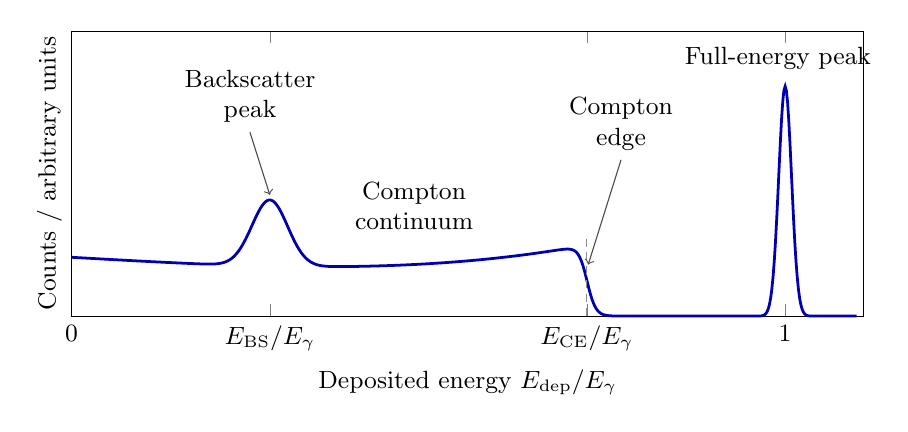
\begin{tikzpicture}
  \begin{axis}[
    width=0.96\textwidth,height=5.2cm,
    xmin=0,xmax=1.11,ymin=0,ymax=1.55,
    xlabel={Deposited energy $E_{\mathrm{dep}}/E_\gamma$},
    ylabel={Counts / arbitrary units},
    xtick={0,0.27778,0.72222,1},
    xticklabels={$0$,$E_{\mathrm{BS}}/E_\gamma$,$E_{\mathrm{CE}}/E_\gamma$,$1$},
    ytick=\empty,
    tick label style={font=\small},label style={font=\small},
    clip=false,
  ]
    % Smooth illustrative continuum and separate illustrative peaks.
    \addplot[blue!70!black,line width=1pt,domain=0:1.1,samples=650]
      {(0.32-0.22*x+0.60*x^3)/(1+exp((x-0.72222)/0.006))
        +0.36*exp(-0.5*((x-0.27778)/0.025)^2)
        +1.25*exp(-0.5*((x-1)/0.009)^2)};
    \draw[black!45,densely dashed] (axis cs:0.72222,0) -- (axis cs:0.72222,0.45);
    \draw[->,black!70] (axis cs:0.25,1.0) -- (axis cs:0.27778,0.66);
    \node[anchor=south,align=center,font=\small] at (axis cs:0.25,1.0)
      {Backscatter\\peak};
    \node[align=center,font=\small] at (axis cs:0.48,0.60)
      {Compton\\continuum};
    \draw[->,black!70] (axis cs:0.77,0.85) -- (axis cs:0.724,0.28);
    \node[anchor=south,align=center,font=\small] at (axis cs:0.77,0.85)
      {Compton\\edge};
    \node[anchor=south,align=center,font=\small] at (axis cs:0.99,1.29)
      {Full-energy peak};
  \end{axis}
\end{tikzpicture}
